\chapter{Core-Collapse Supernovae}
\label{chp:CCSNe}

Supernovae have been witnessed and recorded by humanity for thousands of years. As massively energetic explosions, they can shine brightly in the sky for weeks or months at a time. In 1934, Baade and Zwicky~\cite{baade1934remarks} famously proposed that supernovae might represent the transition of ordinary stars into neutron stars. Over 20 years later, Burbidge et al.~\cite{burbidge1957synthesis} suggested that supernovae might also be important for the synthesis and dissemination of heavy elements. By 1960, Hoyle \& Fowler~\cite{hoyle1960nucleosynthesis} had proposed that there were two main types of supernovae, one involving thermonuclear runaway in degenerate conditions (type Ia), and the other involving the implosion of a stellar core (types II, Ib/c, and hypernovae). The first type occurs when a white dwarf, typically in a binary system, accretes enough mass to reignite carbon fusion~\cite{chen2009progenitors}. This ``runaway nuclear fusion" completely disrupts the star, blowing it apart. This process is believed to be relatively isotropic with no significant asymmetries, and as such, is not expected to emit GWs. Core-Collapse Supernovae (CCSNe) on the other hand are expected to contain significant asymmetries and GW emission.

\begin{figure*}[t]
    \centering
    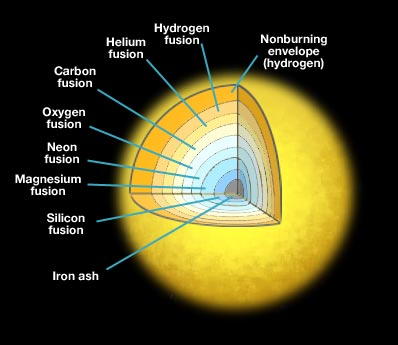
\includegraphics[width=4in]{figures/CCSN_strata.jpg}
    \caption{The stratified distribution of elements in a CCSN progenitor. Figure reproduced from~\cite{strata_source}.}
    \label{fig:CCSN_strata}
\end{figure*}

Near the end of a star's life ($8M_\odot$\,-\,$100M_\odot$~\cite{thesis_jade, janka}) its mass will be distributed by density, with heavier elements near the core and lighter elements composing an outer envelope. This situation is sometimes compared to the layers of an onion and can be seen in Figure~\ref{fig:CCSN_strata}. These stars have enormous gravitational binding energies of order $\sim\,10^{53}$\,ergs~\cite{colgate1966hydrodynamic}. Nuclear burning will cease when the core is composed of iron group nuclei (sometimes ONeMg) and the star becomes gravitationally unstable. When the core reaches the Chandrasekhar mass ($1.44M_\odot$) the electron degeneracy pressure will be overcome and collapse will begin. Eventually the inner core will reach nuclear density and the nuclear equation of state (EoS) will stiffen, causing a shock wave to rebound out radially from the just formed proto-neutron star (PNS). This shock wave will propagate outwards, losing energy via the disassociation of infalling matter and the emission of neutrinos through optically thin regions. The shock wave will quickly stall and become an accretion shock, which must be revived within $\sim$\,0.5\,-\,3 seconds to successfully explode and avoid transitioning directly to a black hole~\cite{thesis_jade}. This shock revival mechanism is still not completely understood and represents one of the biggest unknowns in astrophysics. Gravitational energy is primarily converted to neutrino emission during a CCSN and this offers a possible energy reservoir to revive the shock front. GWs, along with neutrinos, carry information directly from the core of a collapsing star, as opposed to electromagnetic radiation which is only emitted from the outer layers. This means that GWs and neutrinos offer the best opportunities to learn about the inner workings of a CCSN. Contemporary reviews of the CCSN process can be found from Janka~\cite{janka} and M\"uller~\cite{muller2016core}. Subsequent sections in this chapter will detail the core-collapse process, possible revival mechanisms, CCSN asymmetries, detection prospects, and the current state of simulations.

\section{Paths to Core Collapse}

The lifetime of a star is primarily determined by the amount of time it spends in the main sequence (MS) during hydrostatic hydrogen burning. Stars with the appropriate mass to go supernova will typically burn for millions to tens of millions of years~\cite{janka}. When the core is depleted of hydrogen, the star will leave the MS and the evolution of its helium core decouples from that of the stellar envelope. For stars with a sufficiently high central temperature, nuclear fuel can ignite the next burning stage, building up heavier and heavier elements within the inner core. Energy escapes through neutrino losses and the core contracts over time with the occasional respite due to nuclear burning. The actual collapse can occur as nuclear burning ceases or be initiated by a few different processes such as deleptonization and/or photo-disintegration of heavy nuclei~\cite{muller2016core}.

\subsection{Electron-Capture Supernovae}

CCSNe with the smallest progenitor masses are expected to be electron-capture supernovae (ECSNe). These stars have built up oxygen-neon-magnesium (ONeMg) cores through carbon burning~\cite{nomoto1984evolution, nomoto1987evolution, poelarends2008supernova} but reach electron degeneracy before the ignition of neon burning. Electron captures are initiated due to an increasing Fermi level and low reaction thresholds between Ne and Mg~\cite{janka}. The ensuing loss of electron degeneracy pressure results in gravitational collapse. The edge of an ONeMg core has a steep density gradient; after core bounce this results in an accretion shock that expands outward continuously. These conditions are favorable for neutrino-heating, which can further drive the flow of matter away from the core. ECSNe have relatively low masses of 9\,-\,$9.25M_\odot$ for solar-metallicty stars~\cite{poelarends2008supernova}, but that range can shift and widen for lower metallicity progenitors~\cite{pumo2009ec} or for binary systems with mass loss or transfer~\cite{podsiadlowski2004effects}. ECSNe typically explode more often in simulations than their heavier iron-core relatives. Estimates vary, but ECSNe may represent 20\,-\,30\% of all supernovae~\cite{wanajo2009nucleosynthesis, wanajo2010electron}.

\subsection{Iron-core Supernovae}

Stars massive enough to burn Ne will develop an iron core. At temperatures of approximately $10^{10}$\,K the nuclear statistical equilibrium will favor the disassociation of iron-group nuclei into $\alpha$-particles and a growing number of free nucleons~\cite{janka}. This results in contraction, increased density, and increased electron chemical potential. Electron capture further accelerates the collapse as it becomes a run-away process. Iron cores have flatter density profiles compared to ONeMg cores, which results in larger mass accretion rates after bounce and larger ram pressures for the infalling mass. These difficulties mean that sophisticated processes are needed to revive the shock front. Most CCSN simulations that have produced GWs have done so for iron-core progenitors with masses between 11\,-\,$27M_\odot$\,. Normal stellar evolution channels predict a pre-collapse spin period in the tens of seconds or greater~\cite{heger2005presupernova}. Rotation is not expected to play a central role for the majority of CCSNe.

\subsection{Hypernovae and Pair-Instability Supernovae}

Hypernovae (HNe) and Gamma-ray burst (GRB) supernovae are extremely bright events with large ejecta velocities and kinetic energies~\cite{iwamoto1998hypernova}. GRBs are believed to be ultra-relativistic, collimated outflows (``jets") of matter that shoot away from the star. Rapid progenitor rotation and magnetic effects are considered essential for HNe~\cite{woosley2006supernova}. Typically, a HNe is thought of as a rapidly rotating progenitor that collapses directly to a black hole. Energy is emitted via neutrinos, mass flow, and electromagnetic poynting flux. An alternative theory has suggested that a HNe could result from a so-called ``millisecond magnetar", a neutron star with nearly critical rotation and a magnetic field $\geq10^{15}$\,G~\cite{janka}. In either case, rotational and gravitational energy combine to propel ejecta away from the resulting black hole. A high birth spin, alternative stellar evolution path, or binary system is necessary for HNe conditions~\cite{yoon2005evolution, woosley2006progenitor}. HNe are rare and GRBs only accompany an estimated .1\% of supernovae~\cite{janka}.

Pair-instability supernovae (PISNe) are the most massive of all supernovae and have a minimum progenitor mass of $\sim100M_\odot$\,. Such massive stars can encounter the pair-instability at temperatures of order $10^{9}$\,K after central carbon burning~\cite{woosley2002evolution, heger2003heger}. High energy photons produce electron-positron pairs, which converts thermal energy to rest mass energy and lowers the adiabatic index of the nuclear EoS, leading to collapse. PISNe with masses less than $\sim140M_\odot$ and greater than $\sim260M_\odot$ are expected to collapse directly to black holes, while progenitors in between are able to reignite thermonuclear fusion and explode as supernovae. PISNe are rare, with an expected rate of maybe one for every 100\,-\,1000 normal stellar core collapses~\cite{janka}. None of the CCSN GW simulations used in this thesis represent HNe or PISNe.

\section{Shock Revival Mechanisms}
\label{sec:mechanisms}

This section will detail theories related to shock revival in CCSNe with an emphasis on the two predominant models.

\subsection{The Neutrino Model}

It's estimated that 99\% of the energy emitted from a CCSN is in the form of neutrinos~\cite{bethe1990supernova}. Only about 1\% of that would have to be reabsorbed behind the shock front to successfully explode as a supernovae. This idea was first proposed by Arnett~\cite{arnett1966gravitational}, and Colgate \& White~\cite{colgate1966hydrodynamic}. Bethe \& Wilson put the theory in its more modern form~\cite{bethe1985revival}. During the post-bounce accretion phase, hot compacting mass causes the core of the PNS to contract, which leads to increased neutrinospheric temperatures and growing mean energies of radiated neutrinos. The region behind the shock front that primarily absorbs these neutrinos is known as the gain layer, or gain region. A diagram of this scenario can be seen in Figure~\ref{fig:neutrino_model}. Non-radial flows and hydrodynamic instabilities increase the residence time of matter in the gain layer, and thus the total mass in this region~\cite{takiwaki2012three, buras2006two, murphy2008criteria}. This leads to a higher energy deposition rate for neutrinos. Convective overturn and the Standing Accretion Shock Instability (SASI) have both been shown to be important for the success of the neutrino model~\cite{fryer2002modeling, buras2006two, marek2009delayed}. SASI represents oscillations of the expanding shock front, typically modeled as low ($l,m$) modes in a spherical decomposition. These vibrational modes, along with convection, can induce turbulent sloshing and asymmetrical motion in a CCSN.

\begin{figure*}[t]
    \centering
    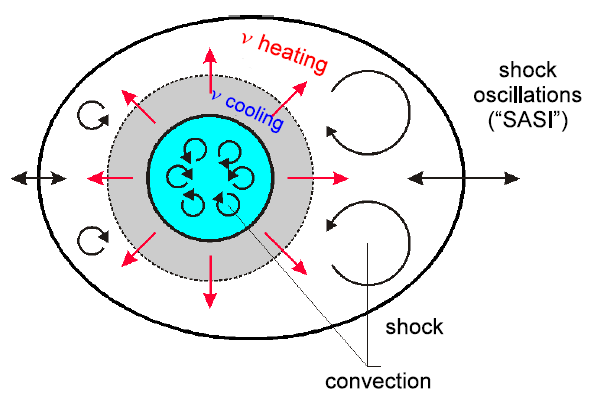
\includegraphics[width=4in]{figures/neutrino_model_diagram.png}
    \caption{Diagram of the neutrino model. Grey coloring represents the accretion layer around the PNS (cyan). Neutrino heating drives convective overturn in the gain region behind the shock front. Picture reproduced from~\cite{muller2016core}.}
    \label{fig:neutrino_model}
\end{figure*}

The GW signals from neutrino model explosions typically contain most of their power between 100\,-1100\,Hz and last between $\sim$\,0.5\,-\,2\,s. Multiple predictable features are present in a typical neutrino model waveform, such as prompt convection after core bounce, low frequency SASI emission below $\sim260$\,Hz, and a g-mode signal that rises in frequency and amplitude~\cite{andresen:16, kuroda:16, 2017arXiv170107325Y}. G-modes use buoyancy as a restoring force and represent oscillations in the PNS. These modes can be instigated from the inner core or at the surface via accreting mass that impinges upon the PNS~\cite{andresen:16, kuroda:16, 2017arXiv170107325Y}. For a source 10\,kpc away, the neutrino model produces a maximum strain of order $\sim10^{-22}$. The total energy emitted in GWs from a neutrino model CCSN is of order $\sim10^{-11}$\,-\,$10^{-9}M_\odot$~\cite{thesis_jade, thesis_josh}. Despite the fact that most simulations still fail to explode, the neutrino model represents the most likely shock revival mechanism in CCSNe.

\subsection{The Magnetorotational Model}

The magnetorotational model was first proposed in the early 1970s~\cite{bisnovatyi1970explosion, ostriker1971pulsars, meier1976magnetohydrodynamic, bisnovatyi1976magnetohydrodynamic} and relies on a rapidly rotating progenitor and highly magnetized PNS. Enormous rotational energy and magnetohydrodynamical (MHD) physics lead to matter being violently expelled away from the star. The initial toroidal component of the magnetic fields for progenitors is predicted to be of order $\sim10^{9}$\,G~\cite{heger2005presupernova}, but simulations have shown that a magnetic field of order $\sim10^{15}$\,G is necessary to power a magnetorotational CCSN~\cite{burrows2007simulations}. This means that magnetic amplification is typically required. The non-radial magnetic field component is expected to increase by a factor greater than $\sim1000$ as mass accretes onto the PNS~\cite{janka}, but further amplification can come from a winding of the poloidal field into the toroidal field. This stretching of the field lines essentially taps into the enormous reservoir of rotational energy. Magnetic fields can also grow exponentially due to the magnetorotational instability (MRI~\cite{balbus1998instability, akiyama2003magnetorotational}) which can grow out of the core~\cite{obergaulinger2009semi}. These amplification processes all require differential rotation, which is a natural result of infall. 

\begin{figure*}[b!]
    \centering
    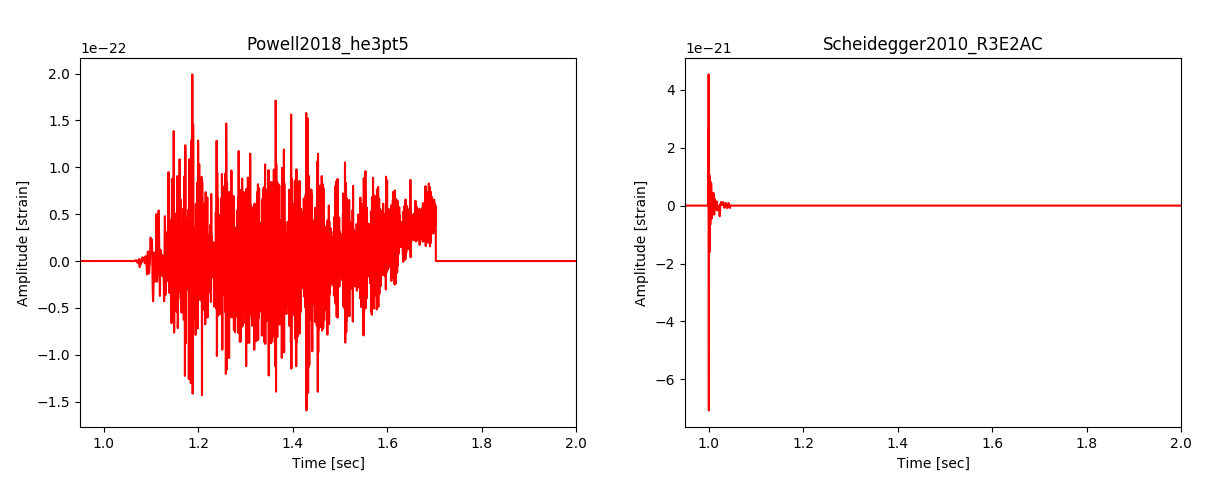
\includegraphics[width=\textwidth]{figures/Two_waveforms_6.png}
    \caption{Example GW signals for the neutrino model (left) and magnetorotational model (right). Core bounce is at t = 1\,s. Neutrino model waveforms typically exhibit sustained, stochastic GW emission, whereas magnetorotational waveforms release their GW energy in a strong burst at core bounce.}
    \label{fig:two_waveforms}
\end{figure*}

It's possible that collimated bipolar jets commonly propel matter along the rotation axis in such CCSN events~\cite{burrows2007simulations, akiyama2003magnetorotational, wheeler2002asymmetric}. The magnetorotational model requires the pre-collapse core to have a spin period less than $\sim2$\,-\,5\,s~\cite{burrows2007simulations, thompson2005viscosity}, which will then experience a frequency ``spin-up" factor of $\sim1000$ after collapse~\cite{ott2006spin}. Stellar evolution models predict that CCSN progenitors will typically have pre-collapse spin periods significantly longer than that~\cite{heger2005presupernova}, potentially even greater than $\sim100$\,s~\cite{janka}. This means that the magnetorotational model requires alternative stellar evolution theories or unusual progenitor birth conditions. It's expected that rapid rotation is present in less than 10\% of progenitor stars~\cite{heger2005presupernova, langer2012presupernova}.

The GW signal from a magnetorotational CCSN is dominated by broadband emission right at core bounce. This spike can be seen in Figure~\ref{fig:two_waveforms}. Rapid rotation causes the core to be deformed by momentum. When the core collapses, the derivatives of the quadrupole moment change significantly and a burst of GWs is emitted. These GWs are heavily dependent on viewing angle and for most magnetorotational simulations the GW energy is primarily found in one component (plus). Other GW features that are commonly found in neutrino model waveforms, such as SASI and g-modes, are less pronounced in rapidly rotating models. This is because rapid rotation can damp convection and because most magnetorotational simulations are short-lived. For a source at 10\,kpc, the magnetorotational model will have a peak strain of $\sim10^{-21}$\,-\,$10^{-20}$ and emit energy in GWs of order $\sim10^{-10}$\,-\,$10^{-8}M_\odot$~\cite{thesis_jade}. The magnetorotational model typically emits more power in GWs than the neutrino model, despite the fact that GWs are only emitted for tens of milliseconds. Most of the power in GWs is between 500\,-\,800\,Hz, but some of the most rapidly rotating models are dominated by centrifugal effects and result in GW emission primarily below $\sim200$\,Hz~\cite{ott2009recent, dimmelmeier2008gravitational}.

\subsection{Other Models}

Other shock revival mechanisms have been proposed, such as the acoustic model~\cite{burrows2007features}. In this model, SASI induces g-modes in the PNS surface. These surface vibrations send large sound waves into the stellar medium. As these waves move down the density gradient away from the PNS they can steepen into secondary shocks that help heat the postshock region and drive the explosion~\cite{janka}. However, 3D simulations have been unable to prove the validity of this mechanism~\cite{marek2009delayed} and a serious counterargument has been proposed against this model~\cite{weinberg2008non}.

Another proposed model is the phase-transition mechanism~\cite{sagert2009signals, fischer2011core}. This model relies on a first-order hadron-to-quark matter phase transition within the core after bounce. As the temperature and pressure rise, the inner core can undergo a transition to pure quark matter. This causes the nuclear EoS to stiffen again, which leads to a second rebounding shock wave that quickly catches up to the first~\cite{sagert2009signals, fischer2011core}. The two core bounces are enough to power the explosion. While this is an interesting theory, the fine-tuning of the quantum chromodynamics (QCD) phase transition is problematic and the hybrid nuclear EoSs that have been used are not compatible with real life stellar observations~\cite{janka}. None of the CCSN GW simulations used in this thesis model the acoustic or phrase-transition mechanisms.

\section{Asymmetries in CCSNe}

Asymmetries are required for the emission of GWs and numerous observations have suggested their presence in CCSNe. The most convincing data comes from measurements of pulsar kicks from recently exploded supernovae, which show average remnant neutron star space velocities of about 400\,km/s and maximum velocities above 1000\,km/s~\cite{hobbs2005statistical}. These values are considered too high to be explained by the breakup of binary systems, which means a natal kick is required~\cite{lai2001pulsar}. Anisotropic emission of gas can only account for neutron star velocities of about 200\,km/s via momentum conservation~\cite{janka1994neutron}. Another way to instigate asymmetrical evolution is to initiate a CCSN simulation with an asymmetrical progenitor~\cite{burrows1996pulsar, arnett2011toward}. Asymmetrical ram pressure can then result in a preferred direction for the explosion to propagate. While this can be effective in simulations, these progenitors are not compatible with our current understanding of stellar evolution models.

Anisotropic neutrino emission is another potential source of asymmetry. An asymmetry of 1\% in the total neutrino energy loss would be sufficient to kick the neutron star to more than 300\,km/s~\cite{janka}. However, the calculated pulsar kicks from anisotropic neutrino emission due to postbounce accetion~\cite{scheck2006multidimensional, wongwathanarat2010hydrodynamical} and convection~\cite{blaschke2001physics} have been estimated to be only $\sim10$\,km/s. It is not fully understood how sufficiently anisotropic neutrino emission would be produced.

Scheck et al.~\cite{scheck2006multidimensional, scheck2004pulsar} proposed the most promising explanation for remnant neutron star velocities. They realized that anisotropically emitted gas would result in long duration anisotropic gravitational forces on the neutron star. They calculated typical final kick velocities in the hundreds of km/s, with extremely anisotropic emission resulting in kick velocities greater than $\sim1000$\,km/s~\cite{scheck2006multidimensional}. This model has been confirmed in 3D~\cite{wongwathanarat2010hydrodynamical}, but the full explanation of where and how this asymmetrical emission originates is not fully understood. The rapid spins of remnant neutron stars is a further complication that is hard to explain without progenitor rotation~\cite{heger2005presupernova, ott2006spin}. Convection, along with hydrodynamical instabilities such as SASI, can establish angular momentum separation between the PNS and ejecta that may lead to significant remnant rotation despite a non-rotating progenitor~\cite{blondin2007pulsar, fernandez2010spiral}. The turbulent motion from SASI and convection is also expected to disrupt the well-stratified onion-shell structure of the progenitor~\cite{kifonidis2006non}, which may contribute to anisotropic emission of gas or neutrinos.

\section{CCSN Rates and Detection Prospects}
\label{sec:rates}

LIGO's initial CCSN search paper~\cite{abbott2016first} estimated the detection efficiency as a function of distance for various models. Pre-dating the advanced detector era, their results were sobering. Neutrino model waveforms had a 50\% detection efficiency at about .2\,kpc, while magnetorotational waveforms had a 50\% efficiency at approximately 1\,kpc~\cite{abbott2016first}. LIGO has recently published their second CCSN search paper based on advanced detector data from O1 and O2. Contemporary detectors are able to detect neutrino model waveforms with a 50\% efficiency at about 2\,kpc, while magnetorotational waveforms had the same efficiency at approximately 20\,kpc.

Estimates of the CCSN rate usually put it between 1\,-\,2 per galaxy per century~\cite{1991ARA&A..29..363V, 1993A&A...273..383C, Alexeyev2002}. If we assume that most CCSN resemble the neutrino model, which is currently the best assumption, then we would need a very nearby galactic CCSN to have any hope of a detection with current detectors. Considering the expected CCSN rate, this is unlikely. Future GW detectors, such as LIGO Voyager~\cite{2015PhRvD..91h2001D, voyagerupgrade}, the Einstein Telescope~\cite{0264-9381-27-19-194002, ET:design}, or LIGO Cosmic Explorer~\cite{2017CQGra..34d4001A, whitepaper2018}, will have drastically reduced noise floors and greatly extended ranges. By the time 3rd generation detectors are operational neutrino model waveforms should be consistently detectable between 100\,-\,150\,kpc, while magnetorotational waveforms should be detectable beyond 600\,-\,700\,kpc~\cite{roma2019astrophysics}. There are a dozen or so known galaxies, mostly satellite or dwarf, within the range of 60 kpc, 28 within the range of 150\,kpc, and 55 within the range of 790\,kpc (the distance to Andromeda)~\cite{karachentsev2004catalog, belokurov2007cats}. As improved detectors come online over the next few decades, a GW detection from a CCSN will become increasingly plausible.

\section{Waveform Simulations}

This section will summarize CCSN gravitational waveforms and models from different simulation groups. 1D and 2D CCSN simulations have been performed for decades and there are many publications exploring the GW emission \cite{muller2004toward, ott2006new, kotake2007gravitational, marek2009equation, yakunin2010gravitational, dimmelmeier2008gravitational}. Simulating a CCSN is famously difficult as multiple forces must be incorporated in an energetically dense and relativistic region of spacetime. Most simulations fail to explode, leading to uncertainty about the shock revival mechanism as described in section \ref{sec:mechanisms}\,. In recent years, advancements have allowed for full 3D simulations that incorporate neutrino physics and general relativity. These simulations have shown modified GW emission from their 2D counterparts but still typically fail to explode. Only 3D CCSN simulations will be presented and used in this thesis. An overview of the CCSN process, including simulation issues and uncertainties, can be found in~\cite{muller2016core}. Figure \ref{fig:example_waveforms} shows example waveforms from each simulation group.

\subsection{Scheidegger}

Scheidegger et al. \cite{scheidegger:10b, scheidegger2010gravitational} produce 25 3D magnetorotational waveforms from a $15M_\odot$ progenitor with varying levels of rotation. The 15 most rapidly rotating models are used in this thesis. The magnetohydrodynamics code of Pen et al.~\cite{pen2003free} and Liebend\"orfer et al.~\cite{liebendorfer2006efficient} is utilized along with two nuclear EoSs, one from Lattimer \& Swesty~\cite{lattimer1991generalized} and one from Shen et al.~\cite{shen1998relativistic}. For the neutrino physics, a parameterized deleptonization scheme is used that incorporates sophisticated computational techniques~\cite{liebendorfer2005simple} but is only valid for a few milliseconds after core bounce.

The GW emission is dominated by a broadband spike at core bounce due to the deformation of a rapidly rotating star and its changing quadrupole moment. Emission continues after bounce but is somewhat reduced due to damped convection in the case of rapid rotation. These simulations are also stopped no later than 130\,ms after core bounce. For these reasons, SASI and g-mode emission is less prominent and won't be considered for magnetorotational waveforms.

\begin{figure*}[p]
    \centering
    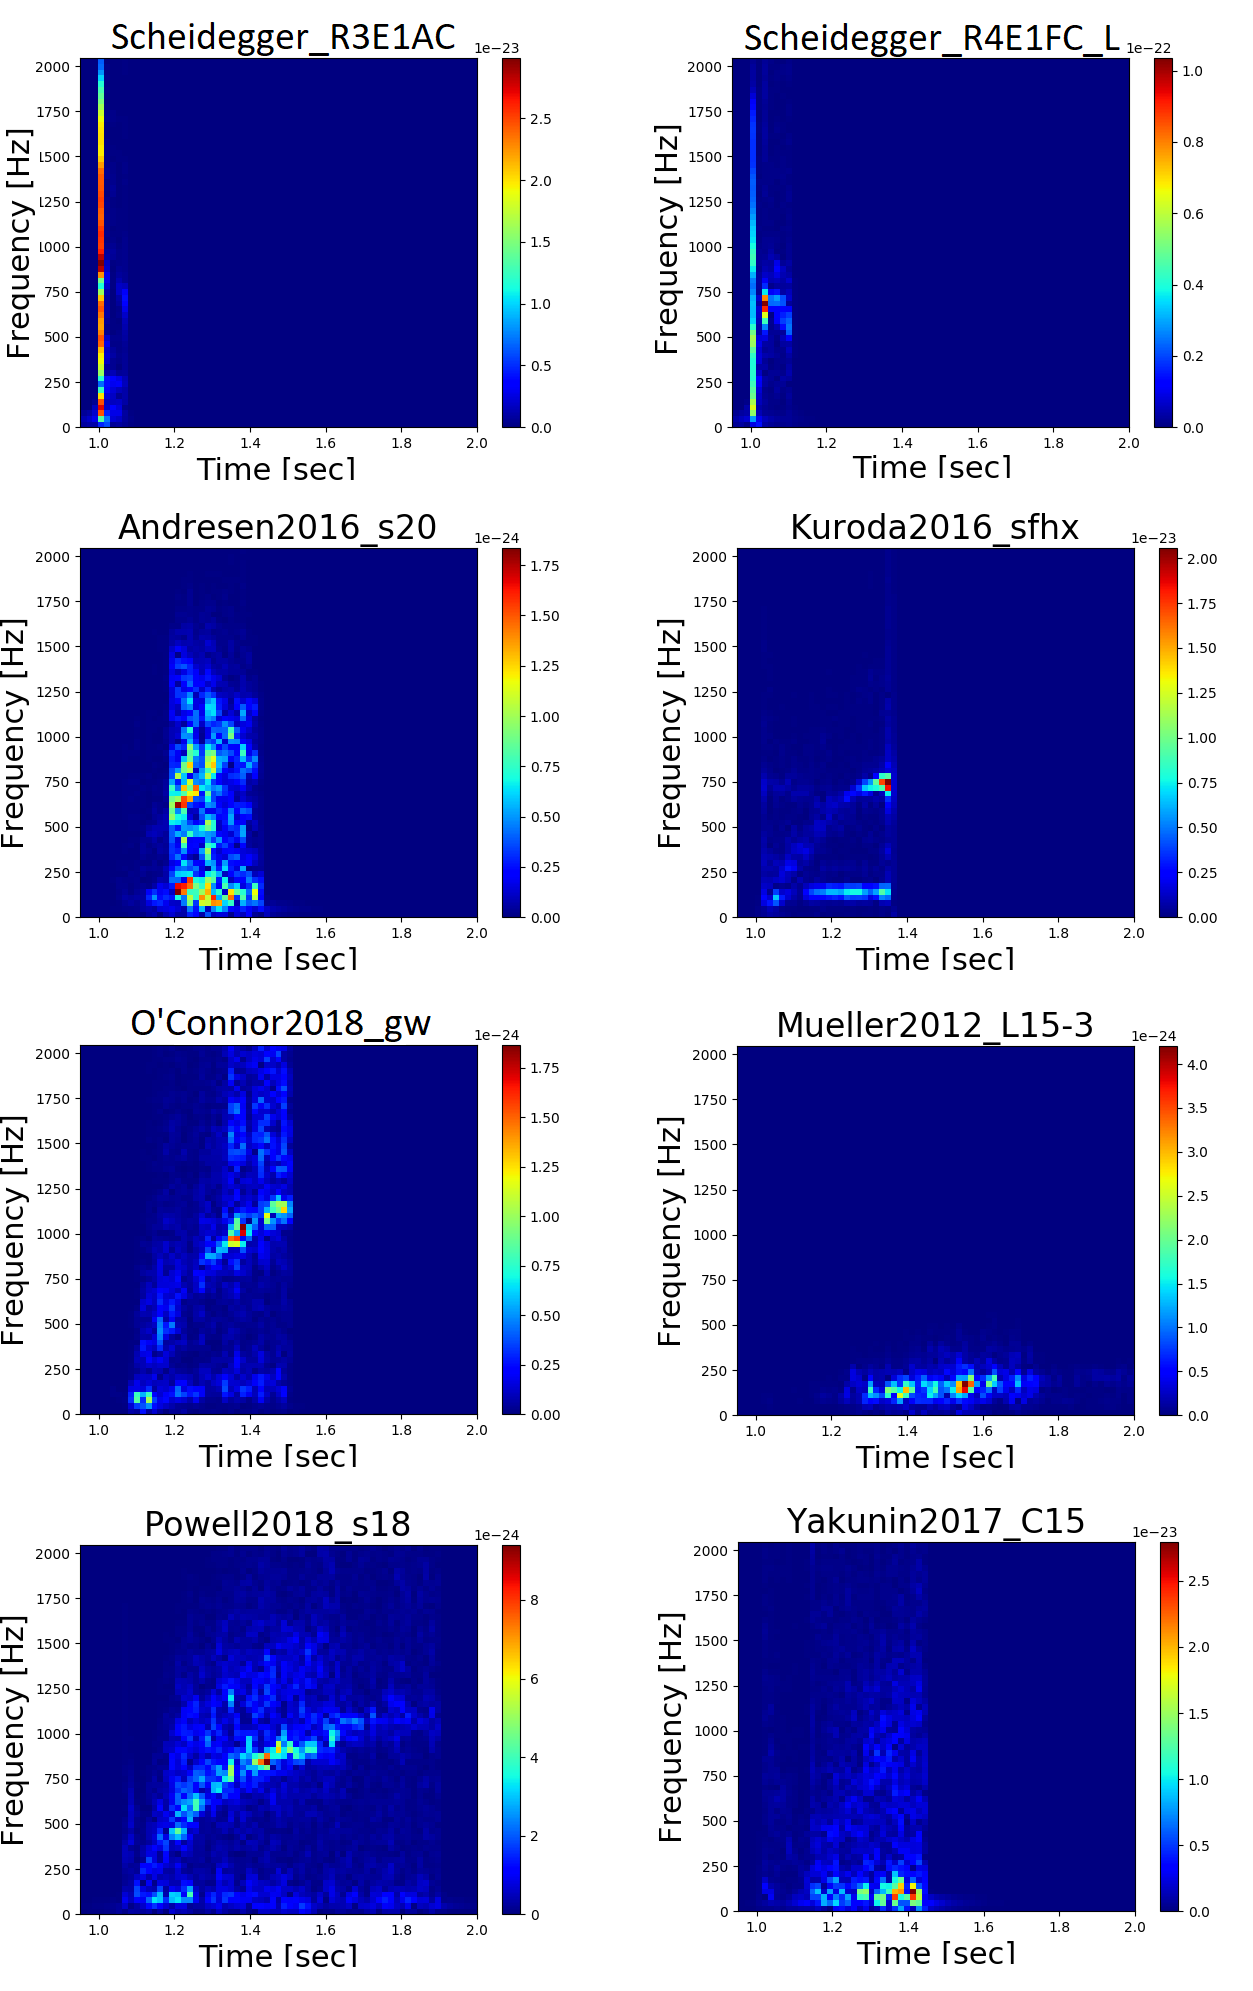
\includegraphics[height=7.9in]{figures/waveform_examples.png}
    \caption{Example waveforms from each simulation group. Two Scheidegger examples are shown as they are the only magnetorotational models used in this thesis. Core bounce is at t = 1\,s in all plots.}
    \label{fig:example_waveforms}
\end{figure*}

\subsection{Andresen}

Andresen et al.~\cite{andresen:16, andresen2018gravitational} have published four simulated neutrino-driven waveforms for non-rotating progenitors. These were 3D multi-group hydrodynamic simulations of progenitors with $11.2M_\odot$ (model s11), $20M_\odot$ (models s20 and s20s), and $27M_\odot$ (model s27). These simulations were created with the PROMETHEUS-VERTEX code~\cite{rampp2002radiation, fryxell1991instabilities}, which combines the Newtonian hydrodynamics module PROMETHEUS~\cite{muller1991instability, fryxell1991instabilities} with the neutrino-transport module VERTEX~\cite{rampp2002radiation}. The effects of general relativity are approximated with a pseudo-relativistic effective potential (case A in~\cite{marek2006exploring}). All four simulations used the Lattimer \& Swesty nuclear equation of state (EoS)~\cite{lattimer1991generalized}.% with a bulk incompressibility modulus for nuclear matter of $K = 220\,$MeV~\cite{lattimer1991generalized}.

Low frequency SASI-related GW emission is significant for all waveforms except model s11. That particular model's shock radius was too large to facilitate the growth of SASI. Instead, its emission is dominated by convection and related high frequency g-modes in the surface of the PNS. This high frequency g-mode emission was present in all four models, but is considered unreliable above 1000\,Hz due to aliasing problems related to the low sampling rate. The duration of the signals varies from 350 ms to 600 ms after core bounce. Model s20s includes modified strange quark interactions for neutral-current neutrino-nucleon scattering~\cite{melson2015neutrino} and was the only model to successfully revive the shock and explode as a CCSN.

\subsection{Kuroda}

Kuroda et al. carry out fully relativistic 3D simulations of a $15M_\odot$ ZAMS progenitor star using three different EoSs~\cite{kuroda:16}. Two of those models, sfhx and tm1, are used in this thesis. They differ from each other in their EoS and treatment of nuclear interactions, with tm1 following~\cite{hempel2010statistical} and sfhx following~\cite{steiner2013core}. Model sfhx is the ``softest" EoS and has the smallest radius. Both models use a $15M_\odot$ star from Woosley \& Weaver~\cite{woosley1995evolution} as the progenitor.

A rising g-mode signal is visible in both Kuroda waveforms. This emission is sourced by oscillations of the PNS surface and grows in frequency over time due to mass accretion. Kuroda et al. find that the growth of SASI is dependent upon the stiffness of the nuclear EoS, with the softest EoS facilitating SASI. Model sfhx therefore has a strong low frequency signal due to sloshing and spiral motions of the SASI, while tm1 does not. Neutrino-driven convection eventually dominates in both models. The simulations were stopped 340\,ms after core bounce.

\subsection{O'Connor/Couch}

This thesis uses 5 neutrino model waveforms from Evan O'Connor and Sean Couch~\cite{o2018exploring}. These simulations use the FLASH hydrodynamics framework that has been outfitted for CCSNe~\cite{couch2013impact, couch2014high}. Multidimensional energy-dependent neutrino-radiation transport based on the moment formalism is included along with effective general relativistic gravity~\cite{o2018two}. All models used a $20M_\odot$ solar metallicity progenitor from Farmer et al.~\cite{farmer2016variations} and the SFHo nuclear EoS from Steiner et al.~\cite{steiner2013core}.

High frequency g-modes were present in every waveform, while late-forming SASI was present in all but one. None of the simulations successfully exploded before being terminated 500\,ms after core bounce. Peak GW emission occurs anywhere from 600\,-\,1250\,Hz in different models. Model v\_LR\_gw differs from other simulations in that it has significant low frequency emission without the formation of SASI. GW emission in this case is reported to be due to turbulent kinetic energy in the gain region.

\subsection{M\"uller}

Three non-rotating neutrino model waveforms are featured from M\"uller et al.~\cite{mueller:e12}. Two of these simulations, models L15 and W15, used $15M_\odot$ progenitors while the other, model N20, used a $20M_\odot$ progenitor. A version of the multi-fluid hydrodynamics code PREMETHEUS~\cite{muller1991instability, fryxell1991instabilities} is once again utilized. Self-gravity is accounted for by solving Poisson's equation in integral form as an expansion into spherical harmonics. The potential's monopole term is corrected for general relativistic effects as described in~\cite{scheck2006multidimensional, arcones2007nucleosynthesis}. ``Ray-by-ray" neutrino transport and neutrino-matter interactions are approximated as in~\cite{scheck2006multidimensional}, while the tabulated EoS from Janka \& M\"uller~\cite{janka1996neutrino} is used to describe the stellar fluid.

Low frequency GW emission was extended as these simulations artificially prescribed the contraction of the PNS. The longest waveform extends to 1.3\,s after core bounce, but the strongest emission happens in the first .7\,s after bounce. Both SASI and g-modes are present in the signals, but the g-modes are slow to develop and rarely approach 300\,Hz. More recent simulations have shown g-mode emission at significantly higher frequencies~\cite{andresen:16, kuroda:16}.

\subsection{Powell}

Powell et .al~\cite{2018arXiv181205738P} carry out two neutrino-driven simulations with the neutrino hydrodynamics code CoCoNut-FMT. A general relativistic finite-volume based solver is used for the equations of hydrodynamics~\cite{muller2010new,dimmelmeier2002relativistic}. As opposed to previous simulations with CoCoNut-FMT, these extended down to the innermost $\sim$ 10\,km to include the PNS convection zone and impose spherical symmetry inside this radius. The neutrino transport is handled using the fast multigroup transport method of M\"uller \& Janka~\cite{muller2015non} with updates to the neutrino rates to be compatible with current experimental constraints and theoretical expectations \cite{hobbs2016role}. The nuclear EoS from Lattimer \& Swesty~\cite{lattimer1991generalized} is used for high density regions. Two models were produced with different progenitors. The first, model he3.5, is an ultra-stripped star in a binary that was evolved from a helium star with an initial mass of $3.5M_\odot$. This is the first GW signal to be produced from an ultra-stripped simulation. The second model used a ZAMS mass of $18M_\odot$ and is referred to as s18.

Both simulations exploded successfully and modelled the emission up to 0.8\,s after core bounce, well into the explosion phase. GW emission is dominated by a surface g-mode induced signal that rises in frequency and peaks between 800\,-\,1000\,Hz. Neither model had SASI activity or significant GW emission at low frequencies.

\subsection{Yakunin}

Yakunin et al.~\cite{yakunin2010gravitational, 2015PhRvD..92h4040Y, 2017arXiv170107325Y} produce one general relativistic, multi-physics, 3D simulation of a $15M_\odot$ progenitor with state of the art weak interactions. The progenitor of Woosley \& Heger~\cite{woosley2007nucleosynthesis} was used and the simulation was carried out with the CHIMERA code, which includes multigroup flux-limited diffusion neutrino transport, and an effective gravitational potential with general relativistic monopole and commensurate corrections to the neutrino transport~\cite{bruenn2016development}. The Lattimer \& Swesty EoS~\cite{lattimer1991generalized} was used for highest density regions and the Cooperstein EoS~\cite{cooperstein1985equation} was used for the lower density regions.

There is a significant quiescent phase after core bounce with little GW emission for 120\,ms. After that point, SASI activity becomes significant and GW emission is instigated. Peak GW emission occurs at about 1000\,Hz due to oscillations in the PSN surface. The simulation is cut off 450\,ms after core bounce. The GW amplitudes in this waveform are significantly larger than those from other simulation groups.

